\documentclass[sigconf,nonacm]{acmart}
\settopmatter{printacmref=false,printfolios=true}
\setcopyright{none}
\renewcommand\footnotetextcopyrightpermission[1]{}
\usepackage{amsmath,tabularx,array,enumitem,tikz,xurl}
\setlength{\emergencystretch}{2em}
\usetikzlibrary{arrows.meta,positioning}
\definecolor{CourseBlue}{HTML}{315EFB}
\definecolor{CourseTeal}{HTML}{14877D}
\definecolor{CourseInk}{HTML}{18324A}
\hypersetup{colorlinks=true,linkcolor=CourseBlue,citecolor=CourseTeal,urlcolor=CourseTeal}
\newcolumntype{Y}{>{\raggedright\arraybackslash}X}
\setlist{topsep=2pt,itemsep=1pt}
\setlist[enumerate]{leftmargin=*}
\setlist[description]{style=nextline,leftmargin=0pt,font=\bfseries}
\title{Compute Commons: Access Rights in Embodied-AI Inference Auctions}
\author{Xinrong Sun}
\affiliation{\institution{Duke Kunshan University}\city{Kunshan}\country{China}}
\email{xs156@duke.edu}
\renewcommand{\shortauthors}{Xinrong Sun, FP9: Compute Commons}
\begin{document}
\begin{teaserfigure}
\centering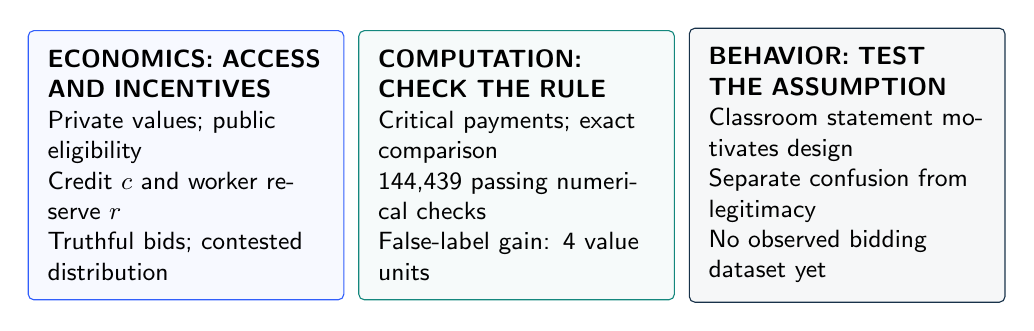
\begin{tikzpicture}[font=\sffamily\small]
\node[draw=CourseBlue,rounded corners=2pt,fill=CourseBlue!4,text width=0.29\textwidth,minimum height=1.55cm,align=left,inner sep=7pt] (a) {\textbf{ECONOMICS: ACCESS AND INCENTIVES}\\Private values; public eligibility\\Credit $c$ and worker reserve $r$\\Truthful bids; contested distribution};
\node[draw=CourseTeal,rounded corners=2pt,fill=CourseTeal!4,text width=0.29\textwidth,minimum height=1.55cm,align=left,inner sep=7pt,right=5pt of a] (b) {\textbf{COMPUTATION: CHECK THE RULE}\\Critical payments; exact comparison\\144,439 passing numerical checks\\False-label gain: 4 value units};
\node[draw=CourseInk,rounded corners=2pt,fill=CourseInk!4,text width=0.29\textwidth,minimum height=1.55cm,align=left,inner sep=7pt,right=5pt of b] (c) {\textbf{BEHAVIOR: TEST THE ASSUMPTION}\\Classroom statement motivates design\\Separate confusion from legitimacy\\No observed bidding dataset yet};
\end{tikzpicture}

\caption{One institutional question, three connected tests. Fixed access rules preserve incentives to report private values, but a false eligibility claim can defeat the access objective. Synthetic calculations establish this boundary; a behavioral pilot and robot measurements remain proposed.}
\Description{Three panels connect private-value bidding, reproducible allocation and payment checks, and a proposed comprehension and legitimacy experiment.}
\end{teaserfigure}
\maketitle\raggedbottom
\noindent\textbf{COMSCI/ECON 206: Computational Microeconomics.} Autumn 2026 Session 1. Instructor: Professor Luyao Zhang.\\
\textbf{FP9: Compute Commons.} Solo team. Review draft, September 27, 2026. Symposium session assignment not supplied.
\section{Shared question and verified gap}
A robot cannot necessarily use computation that it wins: its queued actions may expire, or a moving object may leave the grasp tolerance before inference finishes. The original Compute Commons auction treated inference windows as interchangeable. We instead ask: \emph{Can an access policy allocate usable robot inference while preserving incentives to report private task values?}

\textbf{Economics:} what value and revenue must be traded for entrant access? \textbf{Computation:} how do robot-state constraints change feasible winners? \textbf{Behavior:} do operators distinguish winning compute from receiving a timely action? Their integration changes both the allocation rule and the meaning of access.

Real-time chunking addresses delayed action generation \cite{rtc}; FogROS2 addresses cloud robotics execution \cite{fogros}; deadline-aware task-and-motion planning already allocates reasoning effort \cite{sung}. Themis already auctions GPU resources \cite{themis}. Thus neither latency-aware robotics nor fair compute auctions are new. Our bounded contribution is an inspectable comparison of \emph{nominal versus usable access}, with robot-state ablations and critical payments on a shared feasible set. It is a synthetic mechanism demonstration, not a new control method or a hardware result.

\section{Strategic model and three lenses}
One committed coordinator schedules a batch of robot operators on one inference server. All jobs arrive at time zero. Operator $i$ privately values one timely result at $v_i\geq0$ and submits sealed bid $b_i\geq0$. Public telemetry fixes inference duration $\ell_i$, action-buffer steps $h_i$, control period $\Delta_i$, target speed bound $w_i$, pose tolerance $\epsilon_i$, network delay $\eta_i$ and guard $g_i$. In consistent time units, the usable deadline is
\begin{equation}\label{eq:deadline}
d_i=\min\{h_i\Delta_i,\epsilon_i/w_i\}-\eta_i-g_i.
\end{equation}
For $w_i=0$, the pose bound is infinite. This conservative drift surrogate assumes no predictive compensation. Local control and protective stopping remain outside the auction. Timeliness is necessary, not sufficient, for safe or successful manipulation.

The coordinator commits to horizon $T$, an end-of-horizon worker evaluation reserve $r$, verified entrant status $e_i\in\{0,1\}$ and credit $c\geq0$. Feasible sets $\mathcal F$ admit a nonpreemptive order with completion $C_i\leq d_i$ and $C_i\leq T-r$. Only value is strategically reported. The chosen set maximizes $\sum_{i\in S}(b_i+ce_i)$ over $S\in\mathcal F$, with a fixed tie order. Let $H_i^0$ be the highest rival-score sum over sets excluding $i$, and $H_i^1$ the highest rival-score sum over feasible sets containing $i$. Winners pay
\begin{equation}\label{eq:payment}
p_i=\max(0,H_i^0-H_i^1-ce_i);
\end{equation}
losers pay zero; individually infeasible jobs never win. One sealed deadline, allocation, execution and settlement end the round.

\textbf{Game theory:} utility is $v_ix_i-p_i$, where $x_i$ means timely service. A bid-independent feasible set makes winning monotone and (\ref{eq:payment}) its critical value. Truthful bidding is weakly dominant and hence a Bayesian Nash equilibrium for any private-value prior \cite{harsanyi,roughgarden}. This claim excludes strategic telemetry, status, arrivals, budgets and repeated rounds.

\textbf{Social choice:} firms seek task value, entrants usable access, workers evaluation authority, and the coordinator revenue. Credit is an explicit priority, not measured social benefit. We report task value, revenue, usable entrant access and reserved milliseconds separately. Sen's distinction between resources and opportunities motivates measuring usable access \cite{sen}.

\textbf{Mechanism design:} replace capacity-only admission by robot-state feasibility before charging critical payments. An EDF engineering baseline isolates the value of strategic allocation from the value of respecting deadlines.

\section{Computation and auction comparison}
Enumerate subsets, check each in earliest-deadline-first (EDF) order, maximize credited bids, then compute exclusion/inclusion thresholds. Complexity is $O(2^n n\log n+n^2 2^n)$ for this transparent implementation; it is an offline oracle, not a real-time scheduler. The capacity-only baseline uses the same optimization and EDF dispatch but omits robot deadlines from admission. Its truthful-input outputs are a diagnostic, not an equilibrium in the physical environment. EDF greedily admits feasible jobs by deadline and charges zero.

\begin{table}[h]
\caption{Actual synthetic batch: $T=400$ ms, $\ell_i=200$ ms, $v=(10,9,8,6)$ and $d=(200,200,400,400)$ for $A,B,D,E$. Only $E$ is eligible. Payments follow bidder order within each admitted set.}
\centering\small\setlength{\tabcolsep}{3pt}
\begin{tabular}{lccrr}\toprule
Rule & Admitted & Pays & Value & Rev.\\\midrule
Capacity only & $A,B$ & $8,8$ & 10 & 16\\
EDF & $A,D$ & $0,0$ & 18 & 0\\
Feasible & $A,D$ & $9,6$ & 18 & 15\\
Credit $c=3$ & $A,E$ & $9,5$ & 16 & 14\\
Reserve $r=100$ & $A$ & $9$ & 10 & 9\\
Both $r=100,c=5$ & $E$ & $5$ & 6 & 5\\\bottomrule
\end{tabular}\label{tab:worked}
\end{table}
Capacity-only admission charges $B$ for an expired result, yielding utility $-8$; bidding zero avoids that loss. The feasible rule restores the stated incentive domain. Credit exchanges two value units for one usable entrant result. Removing only buffer expiry or only pose freshness permits $A,B$ and value 19: both physical channels have a consequential role. Reservations reduce usable commercial time; their worker benefit remains unmeasured.

The code verifies 36,289 assertions, including independent permutation checks and unilateral deviations. A paired, seeded sweep of 300 synthetic six-robot batches compares all rules; Appendix A reports means and Monte Carlo intervals. These quantify the chosen input generator, not robot populations. Network-delay stress exposes the fragility of deadlines with no slack.

\section{Behavior and interdisciplinary integration}
The behavioral artifact asks for a bid, predicted payment, predicted timely completion and confidence before showing results. It records regret and a post-outcome explanation. A late baseline winner's underbid may be rational, whereas the same interpretation is unsupported for the verified feasible mechanism. This distinction changes the interface and the behavioral hypothesis; numeric bid error alone is inadequate \cite{hassidim}.

A planned counterbalanced pilot compares a payment tutorial with a physical-deadline explanation. Outcomes are payment error, timeliness prediction and utility regret, with legitimacy judgments measured separately. Learning and distrust remain competing explanations. Manual peer entry supports anonymous local export; it does not provide secure multiplayer bidding. No completed human interactions or classroom causal effects are claimed.

\section{Contribution, practical impact and roadmap}
The proposed case is a shared tabletop pick-and-place testbed used by small integrators and incumbent operators. A shared VLA inference service motivates the workload \cite{openvla}; local controllers handle protective stopping. Log queue depth, object motion, inference/network time and accepted action timestamps to test whether nominal access becomes executable service. Workers select evaluation tasks for the reserved period and can appeal unused capacity. Eligibility and telemetry need independent verification; payments cannot certify safety.

Academia needs calibrated traces and matched baselines; industry needs tail-latency and task-completion evidence; public institutions need usable access and an appeal route. Next: replay measured traces, then controlled robot trials and a preregistered comprehension pilot. Falsify the benefit if calibrated state constraints add no predictive or allocation value. Dynamic coupling, uncertain runtimes, solver latency and multiparameter incentives remain open.

\textbf{2056 aspiration.} Building on Vickrey, Harsanyi, Sen and Pearl \cite{vickrey,harsanyi,sen,pearl}, develop accountable allocation institutions whose incentives, physical feasibility and human effects are independently testable. International research recognition requires generalizable evidence beyond this course prototype.

\textbf{Open science and SDG 4.} Run \texttt{python} \path{code/robot_model.py}; outputs, notebook and source accompany this revision. The \href{https://github.com/dku-comsci-econ206-Autumn2026/-PS2-FP9-ComputeCommons}{course repository} and \href{https://huggingface.co/spaces/dku-comsci-econ206-2026/compute-commons}{Space} are the submission destinations. The intended SDG 4.4 contribution is a reproducible technical-learning exercise, evaluated through explanation accuracy; educational benefit has not been measured.
\IfFileExists{release.tex}{\noindent Computational snapshot: \href{https://github.com/Sunnyxinrong/-PS2-FP9-ComputeCommons/tree/46e71886f36476bd0712d26d4e41e2cfb86db213}{\texttt{46e7188}} (personal fork); \href{https://colab.research.google.com/github/Sunnyxinrong/-PS2-FP9-ComputeCommons/blob/46e71886f36476bd0712d26d4e41e2cfb86db213/code/compute_commons_ps2.ipynb}{runnable notebook}. Team integration and Space revision remain to be confirmed.
}{}

\clearpage
\section*{Author Notes}
\subsection*{Acknowledgments and authorship}
Xinrong Sun is the sole author and selected the original embodied-AI access question, developed the earlier project, and requested this revision after identifying its insufficient robotics specificity. I thank Professor Luyao Zhang for the course framework and supplied templates. The prior proposal records earlier instructor and peer feedback; this revision does not invent new symposium reviews. The cited authors provide the foundations. Python and JavaScript support the computation; the ACM/course templates retain their notices. AI assistance and the verification boundary are recorded below. Authorship and responsibility remain with Xinrong Sun.

\subsection*{Integrated contribution}
Compute Commons connects a resource-allocation institution to an explicit physical service requirement. A robot receives usable access only if inference finishes before its action buffer or pose-validity bound expires. The computational artifact distinguishes capacity-only admission, an engineering deadline baseline, and value-sensitive feasible allocation. The access-credit treatment then exposes the distributional cost within the physically feasible set. Critical payments connect the computation to strategic incentives, while the behavioral interface separates payment prediction from timeliness prediction. Ablations identify which physical assumption changes the result, and a latency stress test limits the interpretation. This integration produces a reproducible synthetic counterexample and a testable research design. It establishes neither real-robot superiority nor an original truthfulness theorem. The same setting, parameters and evidence boundary govern the paper, code, interaction and poster.

\subsection*{Named individual entry: Xinrong Sun, author 1}
\textbf{Intellectual decisions.} Selected embodied-AI compute access and the distinction between consultation and binding access rights in the earlier work. On October 5, identified that interchangeable CPU-like windows did not capture robot specificity and requested a literature-grounded revision. \textbf{Concrete output.} Original proposal and artifacts supplied with this task; revised model in \texttt{code/robot\_model.py}, manuscript Sections 1--5 and behavioral artifact in \texttt{hf\_space/}. \textbf{Verification evidence.} Automated results and source records accompany this revision. The original submission contains the author's review statement for the earlier version; that statement does not establish review of newly generated changes. \textbf{Connection.} The physical definition of usable access changes the economic feasible set, computation and behavioral diagnosis together. \textbf{Next responsibility.} Review and accept or revise this new model, reproduce the key example, verify cited papers, add actual symposium records, and confirm the final submission. Final human review of this revision is not yet recorded.

\bibliographystyle{ACM-Reference-Format}
\bibliography{references}
\appendix
\section{Technical details and reproducibility}
\subsection{Physical model, units and scope}
Each independently operated robot requests one nonpreemptive inference job in a batch released at time zero. No cross-robot collision or task externality is modeled. While it waits, an existing queue executes for $h_i\Delta_i$ ms. With target speed bounded by $w_i$ mm/s and allowed displacement $\epsilon_i$ mm, a constant-bound surrogate permits $1000\epsilon_i/w_i$ ms of observation age. The minimum of these two times, minus network and guard time, is the server completion deadline. Jobs that cannot meet it take an assumed local fallback and obtain zero incremental task value. This is a model of admissible freshness, not a measured grasp-success function, a stability certificate, or a contact dynamics simulator.

OpenVLA motivates shared inference; no OpenVLA checkpoint was executed. RTC motivates the action-queue issue, but its algorithm is not reproduced. Our pose bound is a proposed simplifying assumption, not a theorem or measurement from either paper. Predictive tracking, refreshed observations, variable policy quality and common physical workspaces would change the valuation domain. The admission computation is offline: a deployment must include solver overhead in the time budget and measure worst-case or tail delays.

\begin{center}\small
\begin{tabularx}{\columnwidth}{lY}\toprule
Parameter & Worked instance / interpretation\\\midrule
$n,T,r$ & 4 jobs; 400 ms horizon; reserve 0 or 100 ms at its end.\\
$v$ & $(10,9,8,6)$ for $A,B,D,E$, synthetic private incremental values.\\
$e,c$ & $(0,0,0,1)$; credit 0, 3 or 5 in value units.\\
$\ell,\Delta$ & 200 ms per inference; 100 ms control period.\\
$h$ & $(2,4,4,4)$ queued control steps.\\
$\epsilon,w$ & $(20,10,20,20)$ mm tolerance; 50 mm/s speed for all.\\
$\eta,g$ & Both zero in the worked instance; network delay varied separately.\\
$d$ & $(200,200,400,400)$ ms.\\\bottomrule
\end{tabularx}
\end{center}
All values and telemetry are illustrative. All participants observe the rule and public state but only their own private value. A strategy maps value to one nonnegative sealed bid. A prior is unnecessary for dominant-strategy analysis; any prior over private values yields the stated truthful Bayesian equilibrium. Worker task selection and the coordinator's commitment are institutional assumptions, not additional solved games.

\subsection{Feasibility and incentive argument}
For a fixed subset with all release times zero and deterministic processing times, EDF detects feasibility: swapping an adjacent inverted-deadline pair cannot make either deadline harder to meet when the original order was feasible. Repeated exchanges yield EDF. This claim does not extend unchanged to release times, preemption constraints beyond this model, or sequence-dependent execution times.

Fix rivals' bids and public inputs. The best score among sets containing $i$ is $b_i+ce_i+H_i^1$; the best score excluding it is $H_i^0$. Both $H$ terms are independent of $b_i$. Thus the winning threshold is $H_i^0-H_i^1-ce_i$, subject to the fixed boundary tie rule. Truncate the threshold at zero because bids are nonnegative. Winning at the threshold price gives $v_i-p_i$; losing gives zero. Bidding one's value selects a nonnegative-utility outcome and no unilateral deviation improves it. If no feasible set contains $i$, every report loses. This proves value DSIC, ex-post individual rationality and nonnegative payments under the declared domain using standard critical-payment theory \cite{roughgarden}.

The fixed lexicographic tie rule favors inclusion of earlier bidder indices. Numerical verification does not replace the proof. Credit is a public score offset and creates no cash subsidy. With nonbinding deadlines and identical inference duration, the feasible family is a cardinality constraint and the mechanism reduces to the earlier unit-demand auction. With heterogeneous durations, it generalizes that benchmark to a capacity-constrained subset problem.

\subsection{A strategic counterexample to nominal service}
Capacity-only admission selects $A,B$ and charges 8 each in the worked instance. EDF dispatch gives $A$ completion 200 ms and $B$ completion 400 ms. Since $B$'s deadline is 200 ms, its realized utility is $-8$. Reporting zero removes $B$ and produces utility zero: truthful bidding is not an equilibrium of this diagnostic mechanism when values attach to timely output. Under feasible admission, $A,D$ pay 9 and 6 and obtain utilities 1 and 2. Credit 3 selects $A,E$, paying 9 and 5, each with utility 1. Reserve alone yields utility 1 for $A$; the combined treatment yields utility 1 for $E$. Losers pay zero in all rules.

There is no refund in the deliberately mismatched baseline. Adding contingent refunds defines a different mechanism requiring new incentive analysis. Likewise, physical-state falsification and false eligibility are outside the proof. The inherited model's false-label example remains reproducible in \texttt{code/model.py}; it is a distinct legacy experiment, not a result of the new robot model.

\textbf{Worked strategic representation.} Fix $D,E$ at bids 8 and 6 under the feasible rule, credit zero, and true values $v_A=10,v_B=9$. Restrict the displayed actions to zero and truthful bidding; entries are $(u_A,u_B)$:
\begin{center}\begin{tabular}{lcc}\toprule
 & $b_B=0$ & $b_B=9$\\\midrule
$b_A=0$ & $(0,0)$ & $(0,3)$\\
$b_A=10$ & $(4,0)$ & $(1,0)$\\\bottomrule
\end{tabular}\end{center}
The truthful pair is a Nash equilibrium in this displayed restriction. The earlier threshold argument, not this finite matrix, establishes the full private-type strategy result.

\subsection{Language-independent pseudocode}
\begin{enumerate}
\item Validate finite nonnegative inputs, positive service and control times, binary eligibility, and reserve no greater than horizon.
\item Convert robot state into server deadlines, using an infinite pose bound for a stationary target.
\item Enumerate subsets. Sort each by deadline, then index; accumulate execution time and reject any deadline or horizon violation.
\item Maximize credited bid sum over feasible subsets, resolving equal objectives using the fixed allocation order.
\item For each winner compute best rival score with and without that winner; charge its nonnegative critical value.
\item Evaluate actual completion against physical deadlines. Report value, utility, revenue, nominal/usable access, late jobs and wasted inference time.
\item Repeat with identical inputs for all mechanisms, and independently verify feasibility and unilateral deviations.
\end{enumerate}
The exponential oracle is deliberately limited to at most 12 jobs. Sorting/subset enumeration and repeated threshold scans give the upper bound stated in Section 3. No online scalability claim follows.

\subsection{Actual synthetic sweep and sensitivity}
\begin{center}\small\begin{tabular}{lrrrr}\toprule Rule & Value & Revenue & Entrant & Late\\\midrule
Generic & 21.30 & 14.29 & 0.55 & 2.92\\
EDF & 38.86 & 0.00 & 1.17 & 0.00\\
Feasible & 43.06 & 8.74 & 1.19 & 0.00\\
Credit 3 & 42.99 & 8.43 & 1.26 & 0.00\\
\bottomrule\end{tabular}\end{center}
Feasible minus generic: mean value difference 21.76, paired 95\% Monte Carlo interval [20.05, 23.46].
Feasible minus edf: mean value difference 4.20, paired 95\% Monte Carlo interval [3.50, 4.90].

The generator uses Python's seeded random number generator (seed 206), 300 paired instances, six robots and a 600 ms horizon. Values are discrete uniform integers 1--20. Service time is sampled uniformly from 50, 100, 150 and 200 ms; queue depth from 1--8; tolerance from 10, 20 and 40 mm; speed from 25, 50 and 100 mm/s; network delay from 0, 25 and 50 ms. These quantities are sampled independently. The last two indices are eligible. Credit is 3 and reserve is zero in the random comparison. No parameters were fitted to robot traces.

\begin{sloppypar}
The 95\% intervals are paired mean differences plus/minus $1.96$ standard errors across generated instances. They describe Monte Carlo variability under this arbitrary generator, not external validity or human evidence. Exact feasible optimization weakly dominates any feasible EDF allocation in raw value by construction at zero credit; the comparison measures the size of that modeled opportunity, not a surprising theorem. Revenue for the capacity-only rule includes late-result charges and must not be interpreted as acceptable deployed revenue.
\end{sloppypar}

In the worked ablation, removing queue expiry relaxes $A$ while $B$ remains urgent, and removing pose freshness relaxes $B$ while $A$ remains urgent. Either permits serving both. Removing both gives the generic-capacity special case. Added known network delay of 25 ms invalidates both 200 ms urgent jobs, so feasible admission falls to $D$ only, value 8. This discontinuity is an explicit failure of zero-slack calibration. Unknown execution-time error, variable motion and safety outcomes remain untested.

\subsection{Reproduction and AI-use record}
Run \texttt{python} \path{code/robot_model.py} with Python 3.10 or later (standard library only). It writes \texttt{robot\_results.json} and \texttt{robot\_sweep.csv} beside the source. The notebook embeds the same source for offline execution. \texttt{code/robot-fresh-run.txt} records actual execution. The old \texttt{model.py} and its outputs are retained as explicitly labeled legacy evidence.

\textbf{AI assistance, October 5, 2026.} OpenAI Codex (GPT-6-based agent; exact served model identifier not exposed in this session) assisted after the author's existing project and specific critique. The significant instruction requested a verified robotics literature review, stronger robot-specific modeling, reproducible comparisons and aligned submission artifacts. Material suggestions incorporated into this draft were action-buffer and pose-freshness constraints, feasible-set critical payments, matched scheduling baselines, ablations and revised behavioral questions. It assisted coding, drafting and artifact preparation. Automated checks and source access are recorded separately from human verification. The author's original choices are credited above; acceptance, human edits and final checks of this revision must be recorded by the author before asserting completion. AI is not an author and does not assume scholarly responsibility.

\section{Cumulative intellectual development}
\textbf{Earlier work (supplied source).} PS1 distinguished consultation from binding access. The supplied PS2 draft introduced private values, credits and reservations but explicitly excluded real-time control. Its numerical claims concern interchangeable windows. \textbf{October 5 critique (author).} Robot specificity was insufficient: changing the device label left the mechanism unchanged. \textbf{Revision.} State-derived deadlines now change feasible allocations; raw compute and usable access become distinct metrics. \textbf{Consequence.} The baseline's rationality diagnosis changes when nominal wins have no physical value. Prior files are preserved in the original project directory; this revision has its own source and results.

\section{Verified literature and three-lens checks}
\textbf{RTC \cite{rtc}.} Question: how to execute action chunks despite inference delay. Method: asynchronous chunk generation with inference-time conditioning. Evidence: simulated and real manipulation tasks. Its contribution concerns action continuity and delay robustness. Here, the auction allocates across operators and uses a simple public queue constraint. We neither reproduce RTC nor claim its latency-control insight as original.

\textbf{Deadline-aware task and motion planning \cite{sung}.} Question: how to distribute planning effort under uncertain planning/execution times. Method: an MDP, complexity analysis and approximate search. Evidence: computational experiments. This invalidates a broad novelty claim about deadline-aware robot computation. Our single-batch, deterministic, private-value mechanism instead studies payments and distributive access; the paper supplies no performance benchmark for our auction.

\textbf{FogROS2 \cite{fogros}.} Question: how to execute robot computations on cloud/fog resources. Method: ROS 2 integration and infrastructure selection. Evidence: robotic workloads with measured timing. This motivates measuring network and processing delay separately. Our assumed deterministic delays are not FogROS2 measurements.

\textbf{Themis \cite{themis}.} Question: fair GPU sharing for training workloads. Objective: finish-time fairness and efficiency. Method: auction-based scheduling sensitive to placement. Evidence: workload evaluation. It defeats a claim that fairness and compute auctions are new. Our public physical feasibility and usable entrant-access objective differ; we do not claim superior scheduling to Themis.

\textbf{Vickrey / Myerson framework \cite{vickrey,roughgarden}.} Supplies established incentive theory, not a novel contribution of this project. \textbf{OpenVLA \cite{openvla}.} Supplies application context and published robot-learning evidence; this revision has no trained-policy evaluation. \textbf{Behavior \cite{hassidim}.} Misreporting under strategy-proof matching motivates separating comprehension and beliefs. It does not establish the cause of behavior in our auction.

\textbf{Consequence check.} Game theory forces us to distinguish true timely-service utility from nominal allocation and provides a deviation test. Social choice forces separate usable-access and value metrics and exposes the credit cost. Mechanism design changes admission and payment together. Each affects the same inference decision.

\textbf{Sources and reuse.} Official links and identifiers are in the bibliography. Access date: October 5, 2026. New code implements the model directly and does not import robotics software. The included MIT license covers original code, not third-party course/ACM templates or scholarly works. Source publications were checked through their project, arXiv, publisher or author pages; the review is targeted, not exhaustive. Template notices remain intact. Literature comparison establishes a bounded application gap, not worldwide priority.

\section{Review response and revision record}
\textbf{Revise: author's October 5 comment.} The robot label was interchangeable with generic compute. Changed Sections 1--3, the model, experiment, interface and poster to include queue expiry and pose freshness. Verification: worked counterexample, two channel ablations, EDF comparator and finite incentive tests.

\textbf{Keep: original access question.} Retained entrant priority and worker evaluation rights, but defined the reserve in milliseconds and measured entrant access after physical usability. Cost is reported instead of describing rights as automatically welfare-improving.

\textbf{Investigate: international publication.} Requires calibrated robotics workloads, independent baselines, online compute overhead, actual robot success/fallback measures and a literature search sufficient for the target venue. Synthetic examples alone are insufficient.

\textbf{Symposium evidence not supplied.} The assigned September 28 reviews and author responses were not among the provided records. The old draft calls them future work even though the current revision date is October 5. This revision records the absence of evidence rather than converting those statements into completed reviews. The author must supply the two actual reviews, consequential comments, decisions, changed locations and verification before this course requirement is complete.

\clearpage\onecolumn
\section{Structured abstract and cumulative proposal map}
\begin{table}[h]\small
\begin{tabularx}{\textwidth}{p{0.20\textwidth}Y}\toprule
Element & Current statement\\\midrule
Background & Interchangeable compute rights may fail to provide timely robot actions. Existing scheduling, robotics and incentive theory establish the foundations.\\
Motivation and application & Shared tabletop pick-and-place inference for incumbent and small integrators, with worker-selected evaluation capacity.\\
Connected questions & How do usable access, value and revenue trade off; which physical constraints change allocation; and do people understand timely service and payments separately?\\
Methods and assumptions & Sealed private values, fixed public telemetry and eligibility, deterministic batch scheduling, exact subset maximization and critical payments. Compare generic admission, EDF, feasible auction and access policies.\\
Actual / planned results & Actual synthetic worked value is 10 for generic admission, 18 for feasible admission and 16 with credit 3. Code executes 300 paired instances and 36,289 checks. Robot trials and human pilot remain planned.\\
Intellectual merit & A nominal allocation can defeat both the access objective and the intended value incentive. Public physical feasibility restores the stated incentive domain under a bounded model.\\
Practical impact & Potentially usable access with transparent value costs. Needs verified telemetry, local fallback and an appeal route. No safety, educational or population benefit is established.\\
Feedback and revision & Author's October 5 specificity critique changes the feasible set, metrics and behavioral diagnosis. Earlier files remain available. Actual symposium reviews and final human review remain to be documented.\\\bottomrule
\end{tabularx}
\caption{The same research question and evidence boundary across all revised artifacts.}
\end{table}
\clearpage\twocolumn
\section{PS2 extension: auction and artifact record}
\subsection{Auction laboratory}
Game identifier: \texttt{compute-commons-robot-v2}. The synthetic laboratory uses the four robot states in Appendix A, truthful algorithmic bids $(10,9,8,6)$, fixed index order $A,B,D,E$, and the six treatments in Table~\ref{tab:worked}. Actual results include all payments, utilities, completion times and expiry flags in \texttt{robot\_results.json}. Prediction: truthfulness only for the physically feasible critical-payment rules. The generic diagnostic violates that prediction through negative realized utility. EDF is a nonmarket baseline; its zero payments are not auction revenue evidence.

The interface requires prediction before feedback and allows a facilitator to enter peer bids collected privately beforehand. Local JSON records contain treatment, public inputs, predictions, confidence, own bid, outcome and reflection. No personal names are necessary; no automatic response upload occurs. Synthetic opponents, manual entries and completed human observations must remain distinct. No human dataset accompanies this revision; valid completed-interaction count in the supplied evidence is zero.

\subsection{Artifact parity and release}
The Python oracle, notebook, JavaScript interaction, paper and poster use the same worked profile. The source package retains older evidence clearly labeled as legacy. The formal submission destinations are \url{https://github.com/dku-comsci-econ206-Autumn2026/-PS2-FP9-ComputeCommons} and \url{https://huggingface.co/spaces/dku-comsci-econ206-2026/compute-commons}. The supplied text entry names prior commit \texttt{b03cac82a1b535aa8dbcbd7f1608905386ec5f93}; it must not be represented as containing this revision. Current revision commit and publication status are recorded in the delivered release manifest and text entry.

\subsection{Practical-impact and final-review record}
Course milestones were September 27 (review draft), September 28 (symposium) and September 30 (final revision), 2026. This package is dated October 5 and does not backdate completion. A prospective deployment would allow workers to contest unused reservations and operators to appeal telemetry or eligibility errors. The empirical falsifier is whether measured usable-action rates and value tradeoffs agree with the deadline surrogate under calibrated workloads.

\textbf{Human responsibility.} The research direction and original project are Xinrong Sun's. The author retains responsibility for every submitted claim and artifact. The supplied earlier review statement applies to the earlier files. Final review of the present revision must be completed and recorded by the author; it is not certified by automated verification.

\end{document}
